\chapter{Auswertung}
Wie in der Beschreibung der Versuchsdurchführung erklärt wurden 3 verschiedene Schwingkreise unterschiedlichen Aufbau vermessen. Es werden im Folgenden die Ergebnisse der Messung mit den theoretisch erwarteten Verläufen, die sich aus Kenntnis der Bauelemente ergeben, verglischen.

\section{Analoge Messung}
Mit Hilfe des analogen Oszilloskops wurde nach oben beschriebenem Verfahren ein Reihenschwingkreis vermessen. Als Bauteile kamen zum Einsatz ein Widerstand von $3.3\,$k$\Omega$, eine Spule mit $305.4\,$m$H$ sowie ein Kondensator mit einer Kapazität von $5.01\,$n$F$. Der Messfehler der Durch das nicht komplett präzise Einstellen der Lissajous-Figuren auf das Quadrat am Oszilloskop Bildschirm sowie das Ablesen der Halbachsen entsteht, wurde folgendermaßen abgeschätzt. Beim Ablesen wurde eine Unsicherheit von $0.6\,$mm angenommen und für das Einstellen der Figur wurde eine Unsicherheit im Widerstand von $50\,\Omega$ geschätzt. Die Fehler für den theoretischen Vergleichsverlauf entsteht für den Rest der Arbeit immer dadurch, dass eine relative Unsicherheit bezüglich der elektronischen Werte von 1\% angenommen wird.
\begin{figure}[H]
    \centering
    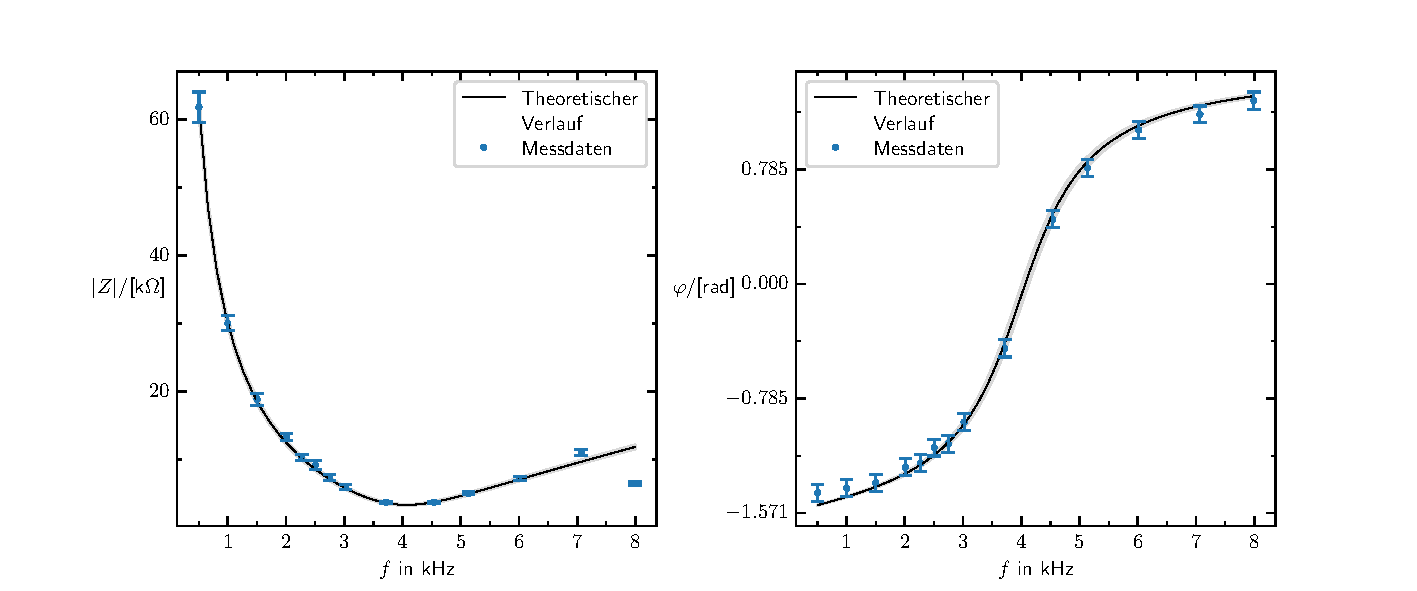
\includegraphics[width = \textwidth]{pictures/analog_reihe.pdf}
    \caption{\textbf{Analoge Messung des Reihenschwingkreises.} Im linken Bild ist der Betrag der Impedanz und im rechten die komplexe Phase der Impedanz eingezeichnet. Der abgeschätzte Fehler der Messungen ist durch die Fehlerbalken angezeigt. Er beträgt die doppelte Standardabweichung. Die Fehler der Theoretischen Kurve ergibt sich immer durch eine 1\% Unsicherheit bezüglich der Kenngrößen der verwendeten Bauteile. Der daraus resultierende Fehler wurde durch einen grau markierten Bereich, der die Kurve umgibt, gekennzeichnet.}
    \label{fig:analog}
\end{figure}
Wie in \figref{fig:analog} zu sehen ist stimmen die gemessenen Werte wirklich gut mit der theoretischen Erwartung überein, die in den meisten Punkten innerhalb der Fehlertoleranz der Messwerte liegt.\vfill\newpage
\section{Digitale Messung}
Die digitale Messung wurde mit Cassy durchgeführt. Es wurde wieder die Impedanz der Schwingkreise ermittelt.
\subsection{Reihenkreis}
Der Reihenschwingkreis, der vermessen wurde, besteht aus einem Widerstand von $3.3\,$k$\Omega$, einer Spule mit $305.4\,$m$H$ sowie einem Kondensator mit einer Kapazität von $22\,$n$F$.
\begin{figure}[H]
    \centering
    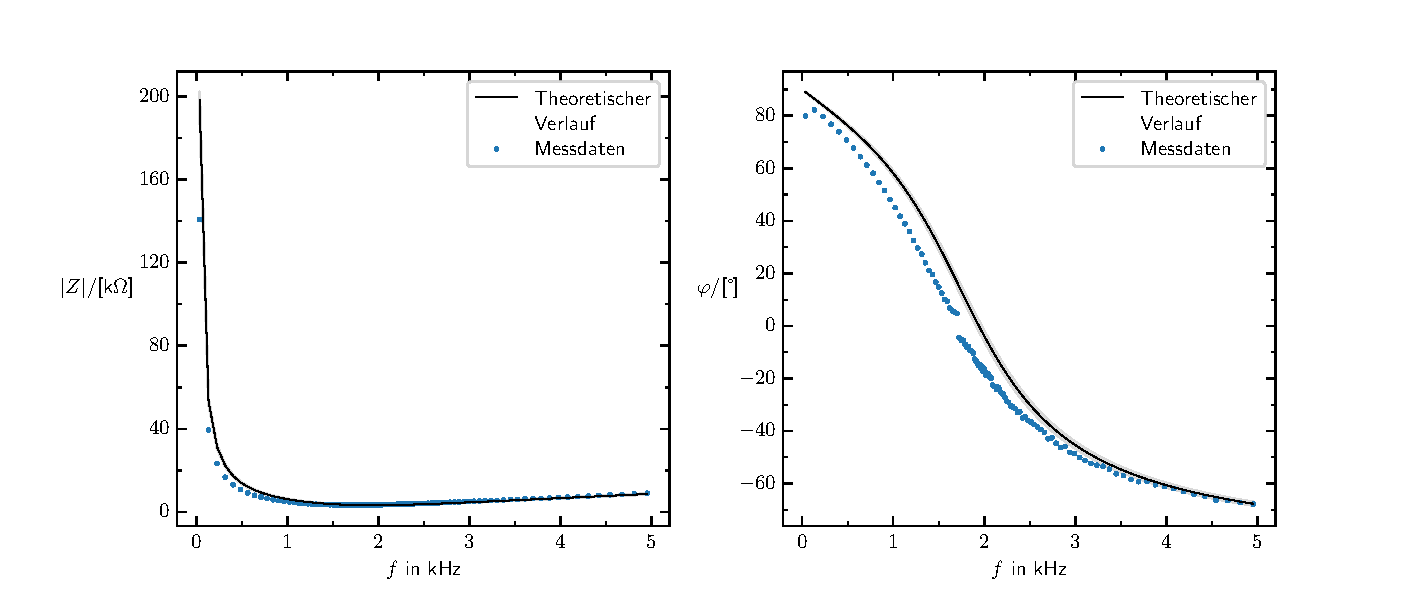
\includegraphics[width = \textwidth]{pictures/digital_reihe.pdf}
    \caption{\textbf{Digitale Messung des Reihenschwingkreises.} Es werden die Messpunkte mit dem theoretisch Erwarteten Verlauf verglichen. Der Fehler für die theoretische Kurve is wieder durch den grauen Bereich gekennzeichnet. Links ist der Betrag und rechts die Phase der Impedanz dargestellt.}
   
\end{figure}

\begin{figure}[H]
    \centering
    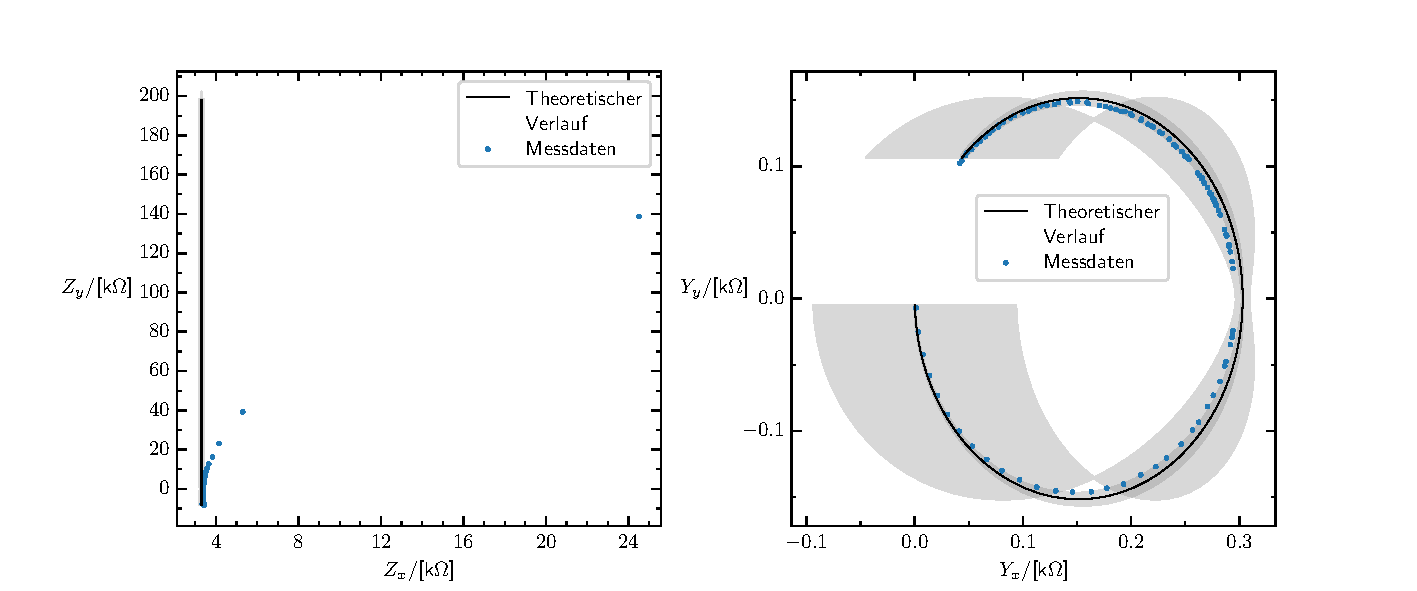
\includegraphics[width = \textwidth]{pictures/digital_reihe_zpolar.pdf}
    \caption{\textbf{Digitale Messung Reihenschwingkreis.} Dargestellt sind Impedanz (rechts) und Admittanz (links) in der Polardarstellung. Da in diesem Fall sowohl die Größe auf der x-Achse also auch die Größe auf der y-Achse für die theoretische Kurve eine Fehler besitzt sind beide Fehler aufgetragen. Wo sich die Fehlerbereiche beider Komponenten überschneiden, ist das Grau der Markierung etwas dunkler, was aber keine Bedeutung hat, und ignoriert werden sollte.}
  
\end{figure}
Man sieht eine leichte Abweichung zwischen Theorie und Messung. Im Schaubild für die Phase bekommt man den Eindruck das möglicherweise ein Offset in die Messung eingeschlichen ist. Die Abweichungen sind auch dadurch beeinflusst, dass die tatsächlichen Werte für die Bauteile leicht von den vom Hersteller angegebenen Werten abweichen. Abweichungen vom erwarteten Verlauf sind besonders deutlich in der Polardarstellung der Impedanz zu beobachten.
% \vfill\newpage
\subsection{Parallelkreis 1. Ordnung}
Der Parallelkreis 1. Ordnung setzte sich in unserem Versuch zusammen aus einem Widerstand mit $22\,$k$\Omega$, einer Spule mit $305.4\,$m$H$ sowie einem Kondensator mit einer Kapazität von $22\,$n$F$. Messung und Experiment sind auch hier wieder gegeneinander verschoben, was die Vermutung eines unberücksichtigten Offsets bestärkt. Es kann auch beobachtet werden, dass die Resonanz in der Messung schwächer ausfällt als die Erwartung. Auch für diesen Schwingkreis sind die Abweichungen zwischen Messung und Theorie am stärksten in der Polardarstellung von Impedanz und Admittanz zu sehen.
\begin{figure}[H]
    \centering
    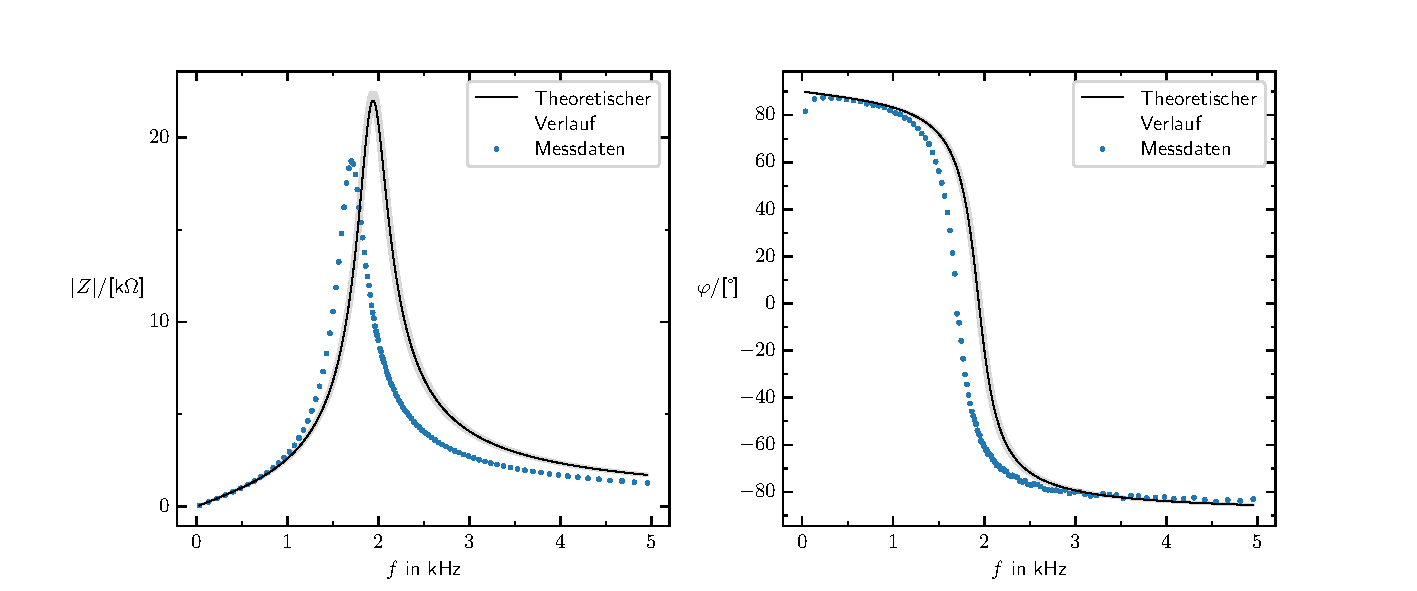
\includegraphics[width = \textwidth]{pictures/digital_par1.pdf}
    \caption{\textbf{Digitale Messung des Parallelkreis 1. Ordnung.} Es werden die Messpunkte mit dem theoretisch Erwarteten Verlauf verglichen. Der Fehler für die theoretische Kurve is wieder durch den grauen Bereich gekennzeichnet. Links ist der Betrag und rechts die Phase der Impedanz dargestellt.}

\end{figure}

\begin{figure}[H]
    \centering
    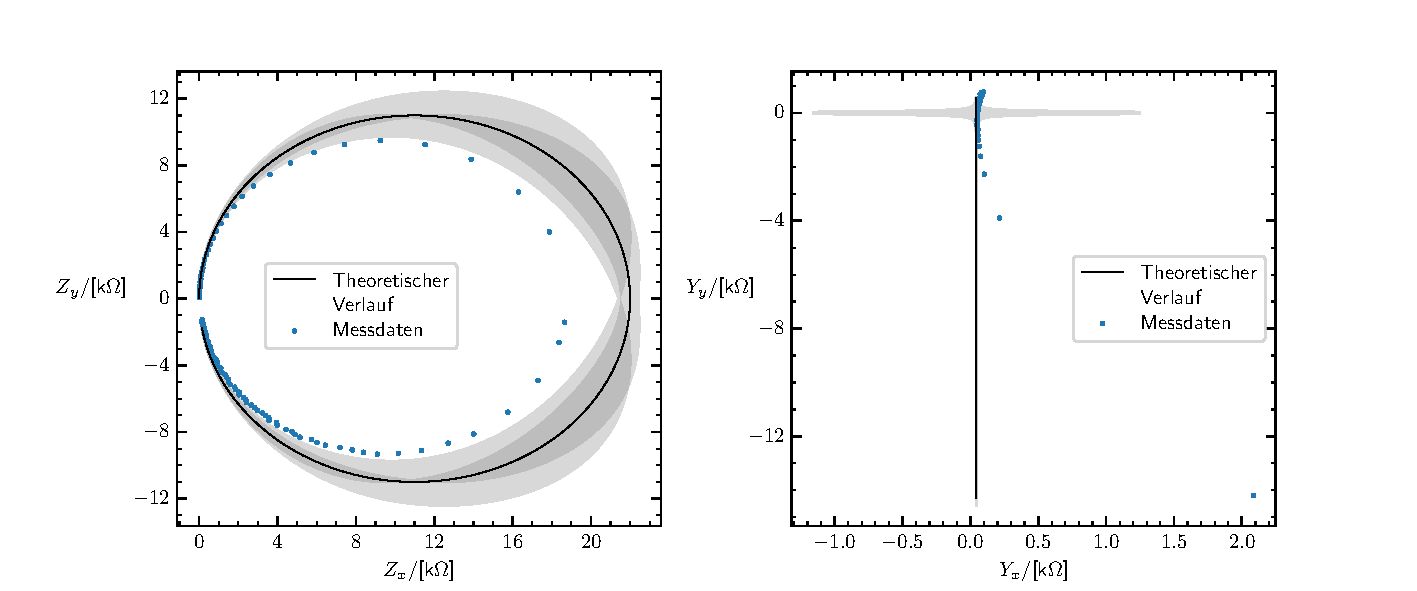
\includegraphics[width = \textwidth]{pictures/digital_par1_zpolar.pdf}
    \caption{\textbf{Digitale Messung Parallelkreis 1. Ordnung.} Dargestellt sind Impedanz (rechts) und Admittanz (links) in der Polardarstellung. Da in diesem Fall sowohl die Größe auf der x-Achse also auch die Größe auf der y-Achse für die theoretische Kurve eine Fehler besitzt sind beide Fehler aufgetragen. Wo sich die Fehlerbereiche beider Komponenten überschneiden, ist das Grau der Markierung etwas dunkler, was aber keine Bedeutung hat, und ignoriert werden sollte.}
   
\end{figure}


\subsection{Parallelkreis 2. Ordnung}
Der Parallelkreis 2. Ordnung besteht aus den Elementen Widerstand ($1.5\,$k$\Omega$), Spule ($305.4\,$m$H$) und Kondensator ($22\,$n$F$). Auch hier beobachtet man eine Verschiebung. Die Resonanz ist um einiges schwächer ausgeprägt als in der Theorie. Auch die Phase hat in der Theorie einen größeren Bewegungsradius. Da die Impedanz allerdings in der Polardarstellung einen weniger perfekten Kreis bildet als in den vorherigen Schwingkreisen, hat sein inverses einen weniger extremen Verlauf. Allerdings sind in diesem Fall die Fehler für die Admittanz teilweise sehr groß.
\begin{figure}[H]
    \centering
    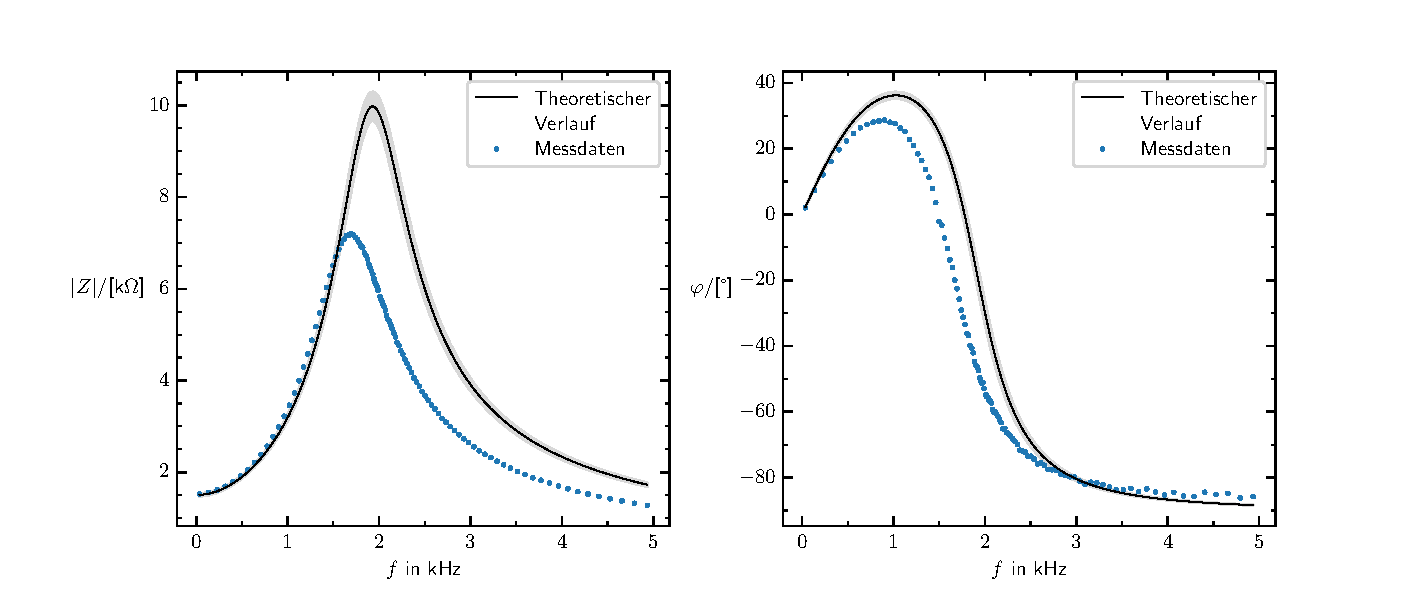
\includegraphics[width = \textwidth]{pictures/digital_par2.pdf}
    \caption{\textbf{Digitale Messung des Parallelkreis 2. Ordnung.} Es werden die Messpunkte mit dem theoretisch Erwarteten Verlauf verglichen. Der Fehler für die theoretische Kurve is wieder durch den grauen Bereich gekennzeichnet. Links ist der Betrag und rechts die Phase der Impedanz dargestellt.}

\end{figure}

\begin{figure}[H]
    \centering
    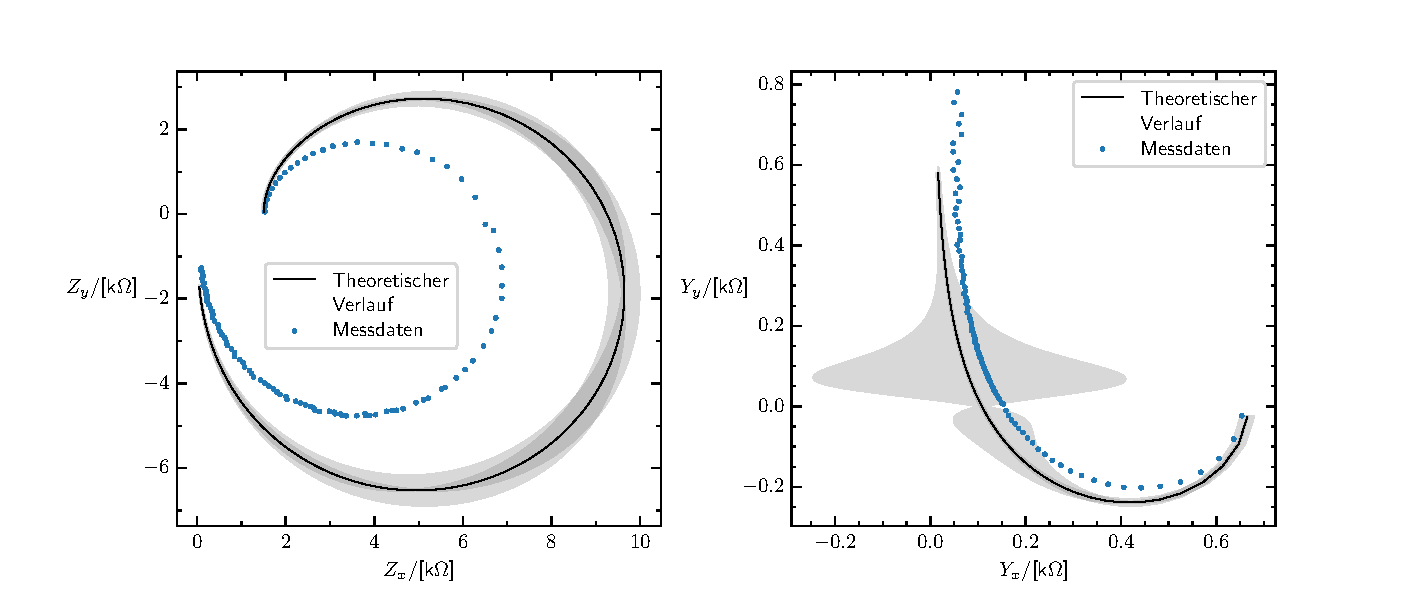
\includegraphics[width = \textwidth]{pictures/digital_par2_zpolar.pdf}
    \caption{\textbf{Digitale Messung Parallelkreis 2. Ordnung.} Dargestellt sind Impedanz (rechts) und Admittanz (links) in der Polardarstellung. Da in diesem Fall sowohl die Größe auf der x-Achse also auch die Größe auf der y-Achse für die theoretische Kurve eine Fehler besitzt sind beide Fehler aufgetragen. Wo sich die Fehlerbereiche beider Komponenten überschneiden, ist das Grau der Markierung etwas dunkler, was aber keine Bedeutung hat, und ignoriert werden sollte.}

\end{figure}